\documentclass[11pt, oneside]{article}

\usepackage{graphicx}
\usepackage{amssymb}
\usepackage{multirow}
\usepackage{float}
\usepackage{amsthm}
\usepackage[left=2cm, right=2cm, top=2cm]{geometry}
\usepackage{array}
\usepackage{pstricks-add}


\theoremstyle{definition}
\newtheorem{exmp}{Example}[section]

\def\rot{\rotatebox}

\begin{document}

\section{What are Natural Numbers?}

Natural Numbers are the first type of numbers that were used historically and are the numbers that are used for counting, which is why they are sometimes called Counting Numbers. The first known use of written numbers is from a carving in bones from approximately 150,000 years ago, which is thought to be used to count and can be seen in the following picture:

\begin{figure}[ht!]
\centering
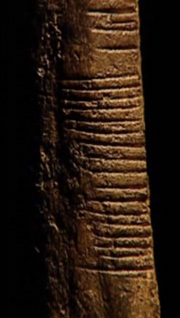
\includegraphics[width=60mm]{bone-carving.jpg}
\caption{Bone carvings used for counting \label{overflow}}
\end{figure}

Numbers evolved and number systems were defined in order to be able to use them more easily and the number system that we use now, which has its origin in India, became the standard system. We also use other numerical systems, for example when counting time, which we will study later on. 

\subsection{Place Value}

Natural numbers and the decimal number system we use are rather convenient to compare and understand the size of numbers. It is important to both understand how numbers are written and what it digit in a number means. For example, let's consider the number 387,542. We can study this number by considering each of its digits:

\begin{tabular}{|c | c | c | c | c | c | c | c |}
\hline
 &  & \rot{90}{Hundred Thousands} & \rot{90}{Tens of Thousands} & \rot{90}{Thousands} & \rot{90}{Hundreds} & \rot{90}{Tens} & \rot{90}{Units} \\ \hline
387,542 & = & 3 & 8 & 7 & 5  & 4 & 2 \\ \hline
\end{tabular}


Let's now look at some examples:

\begin{exmp} \end{exmp}




\subsection{Exercises}
\begin{enumerate}
\item 
\end{enumerate}



\end{document}  




















